% Options for packages loaded elsewhere
% Options for packages loaded elsewhere
\PassOptionsToPackage{unicode}{hyperref}
\PassOptionsToPackage{hyphens}{url}
%
\documentclass[
  11pt,
  ignorenonframetext,
  aspectratio=169,
]{beamer}
\newif\ifbibliography
\usepackage{pgfpages}
\setbeamertemplate{caption}[numbered]
\setbeamertemplate{caption label separator}{: }
\setbeamercolor{caption name}{fg=normal text.fg}
\beamertemplatenavigationsymbolsempty
% remove section numbering
\setbeamertemplate{part page}{
  \centering
  \begin{beamercolorbox}[sep=16pt,center]{part title}
    \usebeamerfont{part title}\insertpart\par
  \end{beamercolorbox}
}
\setbeamertemplate{section page}{
  \centering
  \begin{beamercolorbox}[sep=12pt,center]{section title}
    \usebeamerfont{section title}\insertsection\par
  \end{beamercolorbox}
}
\setbeamertemplate{subsection page}{
  \centering
  \begin{beamercolorbox}[sep=8pt,center]{subsection title}
    \usebeamerfont{subsection title}\insertsubsection\par
  \end{beamercolorbox}
}
% Prevent slide breaks in the middle of a paragraph
\widowpenalties 1 10000
\raggedbottom
\AtBeginPart{
  \frame{\partpage}
}
\AtBeginSection{
  \ifbibliography
  \else
    \frame{\sectionpage}
  \fi
}
\AtBeginSubsection{
  \frame{\subsectionpage}
}
\usepackage{iftex}
\ifPDFTeX
  \usepackage[T1]{fontenc}
  \usepackage[utf8]{inputenc}
  \usepackage{textcomp} % provide euro and other symbols
\else % if luatex or xetex
  \usepackage{unicode-math} % this also loads fontspec
  \defaultfontfeatures{Scale=MatchLowercase}
  \defaultfontfeatures[\rmfamily]{Ligatures=TeX,Scale=1}
\fi
\usepackage{lmodern}

\usetheme[]{metropolis}
\ifPDFTeX\else
  % xetex/luatex font selection
\fi
% Use upquote if available, for straight quotes in verbatim environments
\IfFileExists{upquote.sty}{\usepackage{upquote}}{}
\IfFileExists{microtype.sty}{% use microtype if available
  \usepackage[]{microtype}
  \UseMicrotypeSet[protrusion]{basicmath} % disable protrusion for tt fonts
}{}
\makeatletter
\@ifundefined{KOMAClassName}{% if non-KOMA class
  \IfFileExists{parskip.sty}{%
    \usepackage{parskip}
  }{% else
    \setlength{\parindent}{0pt}
    \setlength{\parskip}{6pt plus 2pt minus 1pt}}
}{% if KOMA class
  \KOMAoptions{parskip=half}}
\makeatother


\usepackage{longtable,booktabs,array}
\newcounter{none} % for unnumbered tables
\usepackage{calc} % for calculating minipage widths
\usepackage{caption}
% Make caption package work with longtable
\makeatletter
\def\fnum@table{\tablename~\thetable}
\makeatother
\usepackage{graphicx}
\makeatletter
\newsavebox\pandoc@box
\newcommand*\pandocbounded[1]{% scales image to fit in text height/width
  \sbox\pandoc@box{#1}%
  \Gscale@div\@tempa{\textheight}{\dimexpr\ht\pandoc@box+\dp\pandoc@box\relax}%
  \Gscale@div\@tempb{\linewidth}{\wd\pandoc@box}%
  \ifdim\@tempb\p@<\@tempa\p@\let\@tempa\@tempb\fi% select the smaller of both
  \ifdim\@tempa\p@<\p@\scalebox{\@tempa}{\usebox\pandoc@box}%
  \else\usebox{\pandoc@box}%
  \fi%
}
% Set default figure placement to htbp
\def\fps@figure{htbp}
\makeatother





\setlength{\emergencystretch}{3em} % prevent overfull lines

\providecommand{\tightlist}{%
  \setlength{\itemsep}{0pt}\setlength{\parskip}{0pt}}



 


\definecolor{navy}{HTML}{23395B}
\definecolor{rust}{HTML}{C8553D}
\definecolor{softgrey}{HTML}{EEF1F5}
\setbeamercolor{frametitle}{bg=navy,fg=white}
\setbeamercolor{progress bar}{fg=rust,bg=softgrey}
\setbeamercolor{alerted text}{fg=rust}
\setbeamercolor{block title}{bg=navy!12,fg=navy}
\setbeamercolor{block body}{bg=navy!4}
\setbeamercolor{block title alerted}{bg=rust!15,fg=rust}
\setbeamercolor{block body alerted}{bg=rust!4}
\setbeamercolor{block title example}{bg=navy!12,fg=navy}
\setbeamercolor{block body example}{bg=softgrey}
\renewcommand{\arraystretch}{1.25}
\newcommand{\ybar}{\bar{y}}
\newcommand{\se}{\mathrm{SE}}
\makeatletter
\@ifpackageloaded{caption}{}{\usepackage{caption}}
\AtBeginDocument{%
\ifdefined\contentsname
  \renewcommand*\contentsname{Table of contents}
\else
  \newcommand\contentsname{Table of contents}
\fi
\ifdefined\listfigurename
  \renewcommand*\listfigurename{List of Figures}
\else
  \newcommand\listfigurename{List of Figures}
\fi
\ifdefined\listtablename
  \renewcommand*\listtablename{List of Tables}
\else
  \newcommand\listtablename{List of Tables}
\fi
\ifdefined\figurename
  \renewcommand*\figurename{Figure}
\else
  \newcommand\figurename{Figure}
\fi
\ifdefined\tablename
  \renewcommand*\tablename{Table}
\else
  \newcommand\tablename{Table}
\fi
}
\@ifpackageloaded{float}{}{\usepackage{float}}
\floatstyle{ruled}
\@ifundefined{c@chapter}{\newfloat{codelisting}{h}{lop}}{\newfloat{codelisting}{h}{lop}[chapter]}
\floatname{codelisting}{Listing}
\newcommand*\listoflistings{\listof{codelisting}{List of Listings}}
\makeatother
\makeatletter
\makeatother
\makeatletter
\@ifpackageloaded{caption}{}{\usepackage{caption}}
\@ifpackageloaded{subcaption}{}{\usepackage{subcaption}}
\makeatother

\usepackage{bookmark}
\IfFileExists{xurl.sty}{\usepackage{xurl}}{} % add URL line breaks if available
\urlstyle{same}
\hypersetup{
  pdftitle={Confidence Intervals \& Hypothesis Testing},
  pdfauthor={TA session · UniTo ESOMAS},
  hidelinks,
  pdfcreator={LaTeX via pandoc}}


\title{\texorpdfstring{Confidence Intervals \& Hypothesis
Testing}{Confidence Intervals \& Hypothesis Testing}}
\subtitle{\texorpdfstring{Econometrics TA session}{Econometrics, TA session}}
\author{27.10.26}
\date{}

\begin{document}
\frame{\titlepage}



\section{1. Warm-up: conditional means}\label{warm-up-conditional-means}

\begin{frame}{Conditional mean: the average \emph{inside a group}}
\protect\phantomsection\label{conditional-mean-the-average-inside-a-group}
\textbf{Idea.} The overall average hides differences between groups. The
conditional mean answers: \emph{``what is the average of \(Y\) among
those with \(X=x\)?''}

\begin{block}{Tiny example}
\protect\phantomsection\label{tiny-example}
10 students. 6 attended the review session (\(X=1\)), 4 did not
(\(X=0\)). Mean grade: \(70\) for attendees, \(55\) for the others.
\[E(Y\mid X=1)=70,\qquad E(Y\mid X=0)=55\]
\end{block}

\begin{itemize}
\tightlist
\item
  In a sample: just the average of the observations in that group.
\end{itemize}
\end{frame}

\begin{frame}{Conditional mean from probabilities (discrete case)}
\protect\phantomsection\label{conditional-mean-from-probabilities-discrete-case}
When we have a joint probability table instead of raw data:

\[\Pr(Y=y\mid X=x)=\frac{\Pr(Y=y,\ X=x)}{\Pr(X=x)}\]
\[E(Y\mid X=x)=\sum_{j} y_j \,\Pr(Y=y_j\mid X=x)\]

\begin{block}{Three-step recipe}
\protect\phantomsection\label{three-step-recipe}
\begin{enumerate}
\tightlist
\item
  \textbf{Pick the row} (or column) of the group \(X=x\).
\item
  \textbf{Divide by its total} \(\Rightarrow\) conditional probabilities
  (they now sum to 1).
\item
  \textbf{Weighted average} of the values \(y_j\) using those
  probabilities.
\end{enumerate}
\end{block}

Same as the ordinary mean, but we first ``zoom in'' on one group and
renormalise.
\end{frame}

\begin{frame}{Law of Iterated Expectations: from groups back to the
whole}
\protect\phantomsection\label{law-of-iterated-expectations-from-groups-back-to-the-whole}
\textbf{Idea.} The overall mean is the \textbf{weighted average of the
group means}, where each group is weighted by \emph{how large it is}.

\begin{block}{Continuing the tiny example}
\protect\phantomsection\label{continuing-the-tiny-example}
\[E(Y)=\underbrace{\tfrac{6}{10}}_{\text{share}}\times\underbrace{70}_{\text{mean}}+\underbrace{\tfrac{4}{10}}_{\text{share}}\times\underbrace{55}_{\text{mean}}=42+22=64\]
\end{block}

\[E(Y)=\sum_{i} E(Y\mid X=x_i)\,\Pr(X=x_i)\qquad\text{in a sample: }\ \bar y=\sum_g \frac{n_g}{n}\,\bar y_g\]

\end{frame}

\begin{frame}{Exercise 1 · Conditional mean from a joint table}
\protect\phantomsection\label{exercise-1-conditional-mean-from-a-joint-table}
A café records, for each customer, the \textbf{number of coffees} \(Y\)
and the \textbf{time of the visit} \(X\). Joint probabilities:

\begin{center}
\begin{tabular}{@{}lrrrr@{}}
\toprule
 & \(Y=0\) & \(Y=1\) & \(Y=2\) & \(Y=3\) \\
\midrule
Morning (\(X=M\))   & 0.06 & 0.18 & 0.24 & 0.12 \\
Afternoon (\(X=A\)) & 0.12 & 0.12 & 0.10 & 0.06 \\
\bottomrule
\end{tabular}
\end{center}

\begin{enumerate}
\item Marginal distribution of \(X\) (add up each row).
\item Conditional distribution of \(Y|X=M\) and \(Y|X=A\) \\
\emph{(hint: divide rows by their total)}.
\item \(E(Y\mid X=M)\) and \(E(Y\mid X=A)\).
\item \(E(Y)\) via the LIE; check against the marginal of \(Y\).
\end{enumerate}
\end{frame}

\begin{frame}[shrink=5]{Solution · Exercise 1}
\textbf{1.} \(\Pr(M)=0.06+0.18+0.24+0.12=\mathbf{0.60}\);
\(\quad \Pr(A)=0.12+0.12+0.10+0.06=\mathbf{0.40}\).

\medskip
\textbf{2.} Divide each row by its total:

\begin{center}
\begin{tabular}{@{}lrrrr@{}}
\toprule
 & \(Y=0\) & \(Y=1\) & \(Y=2\) & \(Y=3\) \\
\midrule
\(\Pr(Y\mid M)\) & 0.10 & 0.30 & 0.40 & 0.20 \\
\(\Pr(Y\mid A)\) & 0.30 & 0.30 & 0.25 & 0.15 \\
\bottomrule
\end{tabular}
\end{center}

\textbf{3.} \(E(Y\mid M)=0(0.1)+1(0.3)+2(0.4)+3(0.2)=\mathbf{1.70}\);
\(\quad E(Y\mid A)=0(0.3)+1(0.3)+2(0.25)+3(0.15)=\mathbf{1.25}\).

\medskip
\textbf{4.} \(E(Y)=E(Y\mid M)\Pr(M)+E(Y\mid A)\Pr(A)=1.70(0.60)+1.25(0.40)=\mathbf{1.52}\).\\
% Check: the marginal of \(Y\) (column sums) is \((0.18,\,0.30,\,0.34,\,0.18)\), so
% \(E(Y)=0.30+0.68+0.54=1.52\) \(\checkmark\).\\
Most customers come in the morning, so \(E(Y)\) lies closer to the morning mean.
\end{frame}


\begin{frame}{Exercise 2 · LIE with group means and sample sizes}
\protect\phantomsection\label{exercise-2-lie-with-group-means-and-sample-sizes}
A survey of 300 students reports average weekly study hours by cohort:

\begin{center}
\begin{tabular}{@{}lrr@{}}
\toprule
Cohort & \(n_g\) & \(\bar y_g\) (hours) \\
\midrule
1st-year Bachelor & 100 & 14 \\
2nd-year Bachelor & 150 & 18 \\
Master & 50 & 26 \\
\bottomrule
\end{tabular}
\end{center}

Compute the average study time of the whole sample, \textbf{without} the
raw data. Then compute the \textbf{unweighted} average of the three
group means: why is it different?

\emph{Hint:} the weights are the group shares \(n_g/n\).
\end{frame}

\begin{frame}{Solution · Exercise 2}
\protect\phantomsection\label{solution-exercise-2}
Weights are \(n_g/n\) = \(1/3,\ 1/2,\ 1/6\):
\[\bar y=\tfrac{100}{300}(14)+\tfrac{150}{300}(18)+\tfrac{50}{300}(26)=4.667+9+4.333=\mathbf{18.0}\text{ hours}\]

The simple average of the group means, \((14+18+26)/3=19.33\), is
\textbf{wrong}: it treats the small Master group as if it were as large
as the others. The LIE needs the \textbf{weights}.
\end{frame}

\begin{frame}{The big picture: why are we doing this?}
\protect\phantomsection\label{the-big-picture-why-are-we-doing-this}
\textbf{The situation.} There is a population with an unknown mean
\(\mu\) (e.g.~the average commuting time of \emph{all} workers). We
cannot measure everybody, so we draw a \textbf{sample} and compute
\(\bar y\).

\textbf{The problem.} A different sample would give a different
\(\bar y\). So \(\bar y\) is only a \emph{guess} of \(\mu\).

\begin{block}{Two questions that statistics answers}
\protect\phantomsection\label{two-questions-that-statistics-answers}
\begin{enumerate}
\tightlist
\item
  \textbf{Confidence interval:} \emph{``Given my sample, which values of
  \(\mu\) are plausible?''} \(\to\) a range instead of a single number.
\item
  \textbf{Hypothesis test:} \emph{``Is a specific claim about \(\mu\)
  (e.g.~\(\mu=30\)) compatible with my sample, or is it too
  surprising?''}
\end{enumerate}
\end{block}
\end{frame}


\section{2. Sampling distribution}\label{sampling-distribution-clt}

\begin{frame}{Why does \(\bar y\) vary? The sampling distribution}
\protect\phantomsection\label{why-does-bar-y-vary-the-sampling-distribution}
\textbf{Thought experiment.} Draw a sample of \(n\) workers, compute
\(\bar y\). Throw it back, draw a \emph{new} sample, compute a new
\(\bar y\). Repeat many times.

\begin{itemize}
\tightlist
\item
  Each repetition gives a \textbf{different} \(\bar y\). So
  \textbf{before} we draw it, \(\bar y\) is a \emph{random variable}.
\item
  The distribution of all these \(\bar y\) values is the
  \textbf{sampling distribution} of \(\bar y\).
\item
  Our actual sample is \textbf{one draw} from that distribution.
  Everything in this session asks: \emph{how far can one draw be from
  \(\mu\)?}
\end{itemize}

\begin{block}{Estimator vs estimate}
\protect\phantomsection\label{estimator-vs-estimate}
\textbf{Estimator} = the recipe (``take the average''), a random
variable. \textbf{Estimate} = the number the recipe gives for
\emph{your} sample.
\end{block}
\end{frame}


\begin{frame}{What we know about the sampling distribution of
\(\bar y\)}
\protect\phantomsection\label{what-we-know-about-the-sampling-distribution-of-bar-y}
For an i.i.d. sample with population mean \(\mu\) and variance
\(\sigma^2\):

\[E(\bar y)=\mu\quad\text{(on average right: unbiased)}\qquad\qquad \mathrm{V}(\bar y)=\frac{\sigma^2}{n}\]

\begin{columns}[T]
\begin{column}{0.52\linewidth}
\begin{figure}[H]

{\centering 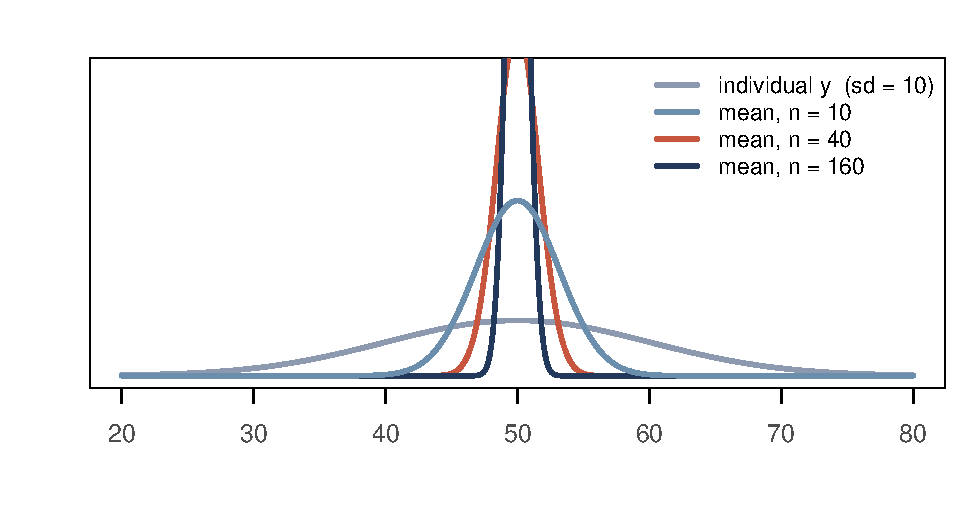
\includegraphics[width=1\linewidth,height=\textheight,keepaspectratio]{figs/se_n.pdf}

}

\caption{Individuals are spread out; sample means are concentrated, more
so as \(n\) grows.}

\end{figure}%
\end{column}

\begin{column}{0.48\linewidth}
\begin{itemize}
\tightlist
\item
  \textbf{Averaging cancels noise:} high and low observations offset
  each other.
\item
  Spread of \(\bar y\) is \(\sigma/\sqrt n\): \(n=10,40,160\) gives
  \(3.2,\ 1.6,\ 0.8\) (with \(\sigma=10\)).
\end{itemize}
\end{column}
\end{columns}
\end{frame}


\begin{frame}{Estimating the unknown: \(s^2\) and the standard error}
\protect\phantomsection\label{estimating-the-unknown-s2-and-the-standard-error}
We almost never know \(\sigma\). We replace it by the sample version:

\[s_{n-1}^2=\frac{1}{n-1}\sum_{i=1}^n (y_i-\bar y)^2 ,\qquad\qquad \hat{V}(\bar y)=\frac{s^2_{n-1}}{n}\]

\begin{itemize}
\item
  \textbf{Why \(n-1\)?} The deviations are measured from \(\bar y\),
  which was itself fitted to \emph{these} data, so they are slightly too
  small. Dividing by \(n-1\) (``degrees of freedom'': one is used up by
  \(\bar y\)) corrects it exactly on average.
\end{itemize}
\end{frame}

% \begin{frame}{Central Limit Theorem: why everything works}
% \protect\phantomsection\label{central-limit-theorem-why-everything-works}
% \begin{figure}[H]
% {\centering 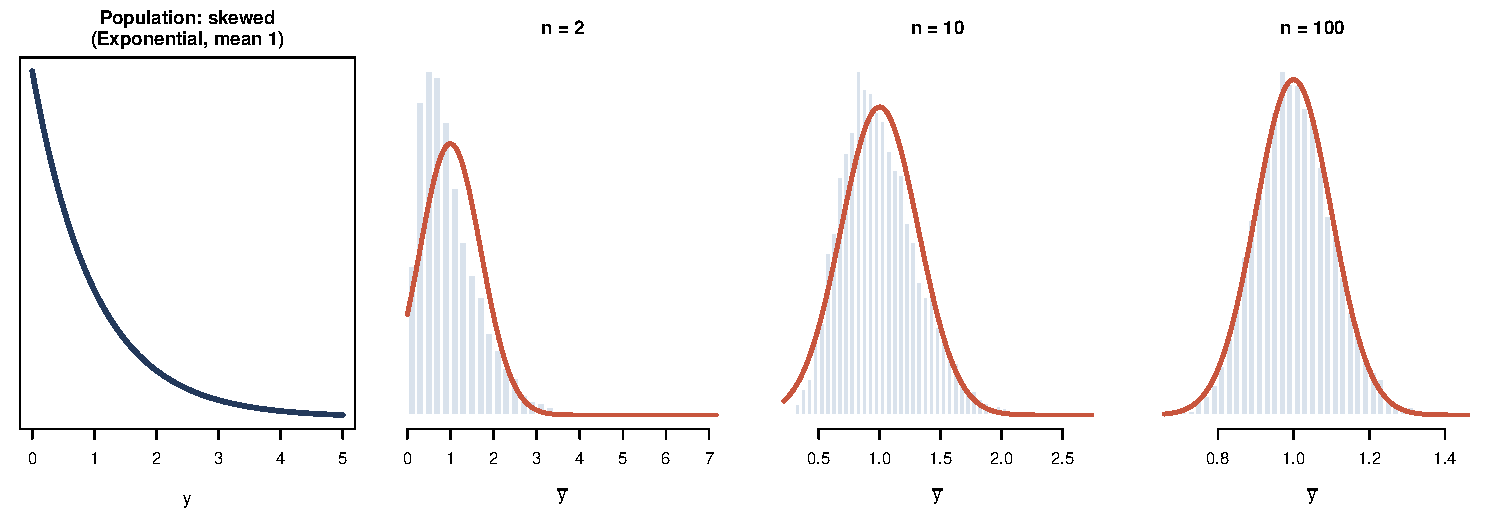
\includegraphics[width=0.85\linewidth,height=\textheight,keepaspectratio]{figs/clt.pdf}
% }
% \caption{Sampling distribution of \(\bar y\) from a skewed population;
% red = \(N(\mu,\sigma^2/n)\)}
% \end{figure}%
% \begin{block}{In words}
% \protect\phantomsection\label{in-words}
% Even if individual data are far from bell-shaped, the \textbf{average}
% of many of them \emph{is} bell-shaped, centred at \(\mu\) with sd
% \(\sigma/\sqrt n\). This is what lets us use normal-table numbers (like
% 1.96) for any reasonable data, as long as \(n\) is large.
% \end{block}
% \end{frame}

\begin{frame}{Exercise 3: Sample variance and standard error}
\protect\phantomsection\label{exercise-3-sample-variance-and-standard-error}
A sample of \(n=26\) daily sales figures has
\(\sum_{i=1}^{26}(y_i-\bar y)^2=1000\).

\begin{enumerate}
\tightlist
\item
  What is the sample variance \(s^2_{n-1}\)?
\item
  What is the standard error of \(\bar y\)?
\item
  Which of these is a common wrong answer, and what mistake produces it? \\
  (a) \(1.240\) \(\quad\) (b) \(1.538\) \(\quad\) (c)
  \(6.325\) \(\quad\) (d) \(38.46\) \(\quad\) (e) \(40\)
\end{enumerate}

\emph{Hint:} divide by \(n-1\) first, then divide by \(n\), then take
the square root.
\end{frame}


\begin{frame}{Solution Exercise 3}
\protect\phantomsection\label{solution-exercise-3}
\begin{enumerate}
\item
  \(s^2_{n-1}=\dfrac{1000}{n-1}=\dfrac{1000}{25}=\mathbf{40}\) (divide
  by \(n-1\), not \(n\)).
\item
  \(\se(\bar y)=\sqrt{\dfrac{s^2_{n-1}}{n}}=\sqrt{\dfrac{40}{26}}=\sqrt{1.538}=\mathbf{1.240}\)
  \(\to\) \textbf{(a)}
\item
  The traps:

  \begin{itemize}
  \tightlist
  \item
    \begin{enumerate}
    [(a)]
    \setcounter{enumii}{1}
    \tightlist
    \item
      \(1.538=s^2/n\): forgot the square root
    \end{enumerate}
  \item
    \begin{enumerate}
    [(a)]
    \setcounter{enumii}{2}
    \tightlist
    \item
      \(6.325=s\): forgot to divide by \(\sqrt n\) (that is the sd, not
      the SE)
    \end{enumerate}
  \item
    \begin{enumerate}
    [(a)]
    \setcounter{enumii}{3}
    \tightlist
    \item
      \(38.46=1000/26\): divided by \(n\) instead of \(n-1\) (and no
      root)
    \end{enumerate}
  \item
    \begin{enumerate}
    [(a)]
    \setcounter{enumii}{4}
    \tightlist
    \item
      \(40\): that is \(s^2\), not the SE
    \end{enumerate}
  \end{itemize}
\end{enumerate}
\end{frame}

\section{3. Confidence intervals}\label{confidence-intervals}

\begin{frame}{From a point estimate to an interval}
\protect\phantomsection\label{from-a-point-estimate-to-an-interval}
\textbf{Idea.} \(\bar y\) is a single guess. We know it is typically off
by about one standard error, so we report a range around it:

\[\boxed{\ \text{estimate}\ \pm\ \text{(multiplier)}\times\text{(standard error)}\ }\]

\begin{itemize}
\tightlist
\item
  \textbf{Standard error} = how noisy our estimate is.
\item
  \textbf{Multiplier} (critical value) = how \emph{confident} we want to
  be. More confidence \(\Rightarrow\) bigger multiplier \(\Rightarrow\)
  wider interval.
\end{itemize}

\begin{block}{Why is the multiplier 1.96 for 95\%?}
\protect\phantomsection\label{why-is-the-multiplier-1.96-for-95}
If \(\bar y\) is normal around \(\mu\), then \textbf{95\% of the time}
it falls within \(\pm1.96\) standard errors of \(\mu\) (figure on the
next slide). So \(\mu\) is within \(\pm1.96\) SE of \(\bar y\) in 95\%
of samples.
\end{block}
\end{frame}

\begin{frame}{Where 1.96 comes from}
\protect\phantomsection\label{where-1.96-comes-from}
\begin{figure}[H]

{\centering 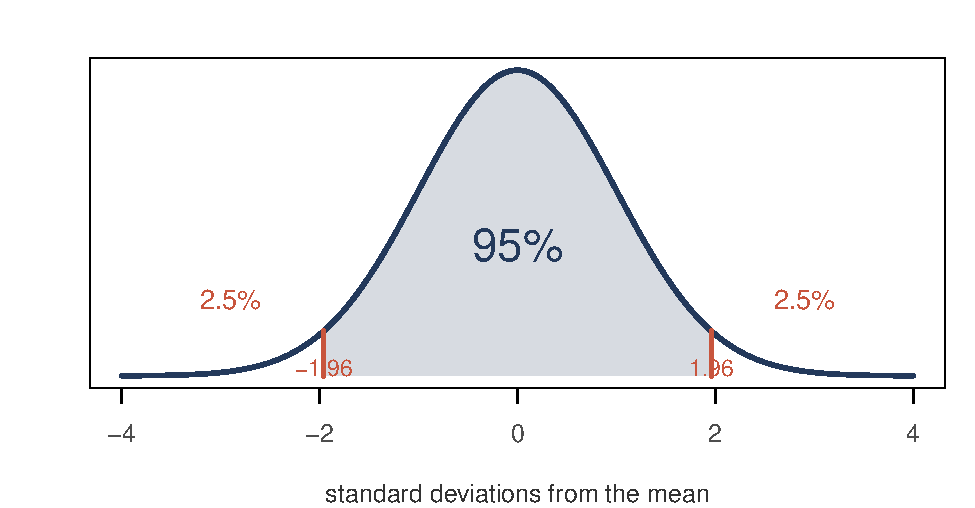
\includegraphics[width=0.55\linewidth,height=0.45\textheight,keepaspectratio]{figs/normal95.pdf}
}
\caption{The central 95\% of a standard normal lies within \(\pm1.96\).
Leaves 2.5\% in each tail.}
\end{figure}%

\begin{itemize}
\tightlist
\item
  Notation: confidence level \(=1-\alpha\). For 95\%, \(\alpha=0.05\),
  split equally between the two tails.
\item
  The multiplier is \(z_{1-\alpha/2}\): for 95\% we need the
  \textbf{0.975 quantile} (leaving 2.5\% in the upper tail).
\item
  90\% \(\to\) \(\pm1.645\) \(\qquad\) 95\% \(\to\)
  \(\pm1.960\) \(\qquad\) 99\% \(\to\) \(\pm2.576\)
\end{itemize}
\end{frame}

\begin{frame}{Deriving the interval (known \(\sigma\))}
\protect\phantomsection\label{deriving-the-interval-known-sigma}
With \(z=z_{1-\alpha/2}\), we start from what we know about the
standardised mean, \(\dfrac{\bar y-\mu}{\sigma/\sqrt n}\sim N(0,1)\), and
rearrange to isolate \(\mu\):
\[\Pr\!\left(-z\le\frac{\bar y-\mu}{\sigma/\sqrt n}\le z\right)=1-\alpha
\ \Longleftrightarrow\
\Pr\!\left(\bar y-z\tfrac{\sigma}{\sqrt n}\le\mu\le\bar y+z\tfrac{\sigma}{\sqrt n}\right)=1-\alpha\]

\begin{block}{The \((1-\alpha)\) confidence interval}
\[\bar y\ \pm\ z_{1-\alpha/2}\,\frac{\sigma}{\sqrt n}\]
\end{block}

\begin{itemize}
\tightlist
\item
  Look at what is random in the second probability: \textbf{not}
  \(\mu\) (a fixed number), but the endpoints, because they contain
  \(\bar y\).
\end{itemize}
\end{frame}

\begin{frame}[shrink=1]{But we don't know \(\sigma\): which distribution?}
\protect\phantomsection\label{which-distribution-does-the-standardised-mean-follow}
Standardising = ``how many standard errors away from \(\mu\) is
\(\bar y\)?'' Replacing \(\sigma\) by \(s\) changes the answer:

{\renewcommand{\arraystretch}{2}
\begin{tabular}{@{}lcl@{}}
  \toprule
  Situation & Statistic & Distribution \\
  \midrule
  $\sigma^2$ \textbf{known}, $Y$ normal
    & $\dfrac{\bar y-\mu}{\sigma/\sqrt n}$     & $N(0,1)$ \textbf{exactly} \\
  $\sigma^2$ \textbf{known}, $Y$ any, $n$ large
    & $\dfrac{\bar y-\mu}{\sigma/\sqrt n}$     & $\approx N(0,1)$ (CLT) \\
  $\sigma^2$ \textbf{unknown}, $Y$ normal
    & $\dfrac{\bar y-\mu}{s_{n-1}/\sqrt n}$    & $t_{n-1}$ \textbf{exactly} \\
  $\sigma^2$ \textbf{unknown}, $Y$ any, $n$ large
    & $\dfrac{\bar y-\mu}{s_{n-1}/\sqrt n}$    & $\approx N(0,1)$ (CLT) \\
  \bottomrule
\end{tabular}}

\smallskip
\begin{itemize}
\tightlist
\item
  \textbf{Why \(t\) in the third row?} \emph{two} sources of uncertainty: \(\bar y\) is random \textbf{and} \(s\) is random. The \(t\) distribution has fatter tails to account for the extra uncertainty.
\item
  \textbf{Small \(n\) needs normal data}; large \(n\) is rescued by the CLT.
\end{itemize}
\end{frame}

\begin{frame}[shrink=6]{What does ``95\% confident'' really mean?}
\protect\phantomsection\label{what-does-95-confident-really-mean}
\begin{columns}[T]
\begin{column}{0.48\linewidth}
\begin{itemize}
\tightlist
\item
  A CI is a \textbf{random interval}: its endpoints are statistics, so
  each sample gives a different one.
\item
  It contains the unknown \(\mu\) with the \textbf{preassigned
  probability} \(1-\alpha\). For 95\%: about 95 intervals out of 100
  contain \(\mu\).
\end{itemize}

% \begin{alertblock}{Common mistake}
% \small Once computed, e.g.~\([19.02,\ 20.98]\), the interval either contains
% \(\mu\) or it does not. ``There is a 95\% probability that \(\mu\) is
% in \([19.02,\ 20.98]\)'' is \textbf{wrong}: the 95\% describes the
% \emph{procedure}, not this one interval.
% \end{alertblock}
\end{column}

\begin{column}{0.52\linewidth}
\begin{figure}[H]

{\centering 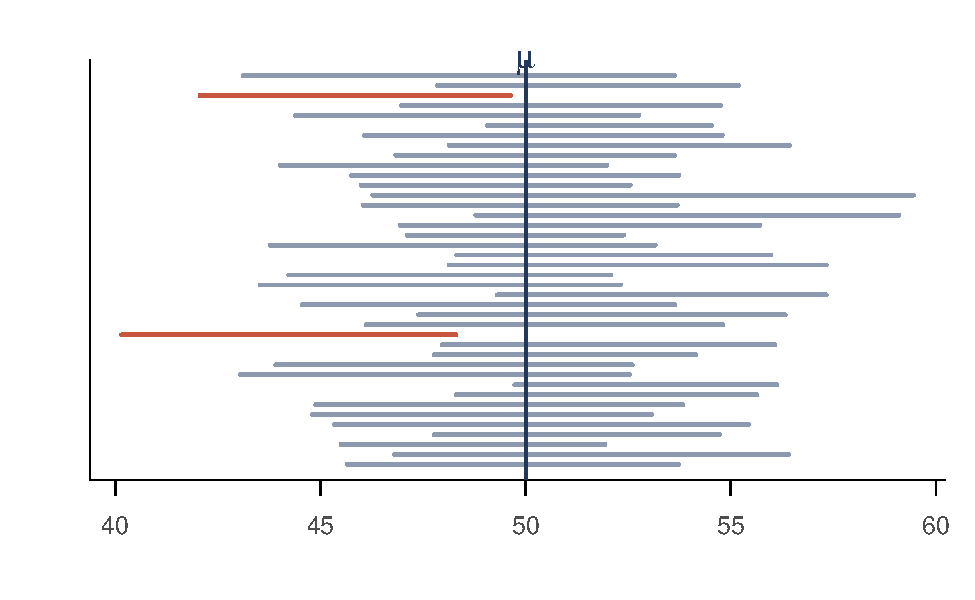
\includegraphics[width=1\linewidth,height=\textheight,keepaspectratio]{figs/ci_coverage.pdf}

}

\caption{40 samples, 95\% CIs. Red = interval misses \(\mu\) (about 1 in
20).}

\end{figure}%
\end{column}
\end{columns}
\end{frame}



\begin{frame}{\(z\) or \(t\)?}
\protect\phantomsection\label{z-or-t-which-table-do-i-open}
\begin{columns}[T]
\begin{column}{0.55\linewidth}
\begin{figure}[H]

{\centering 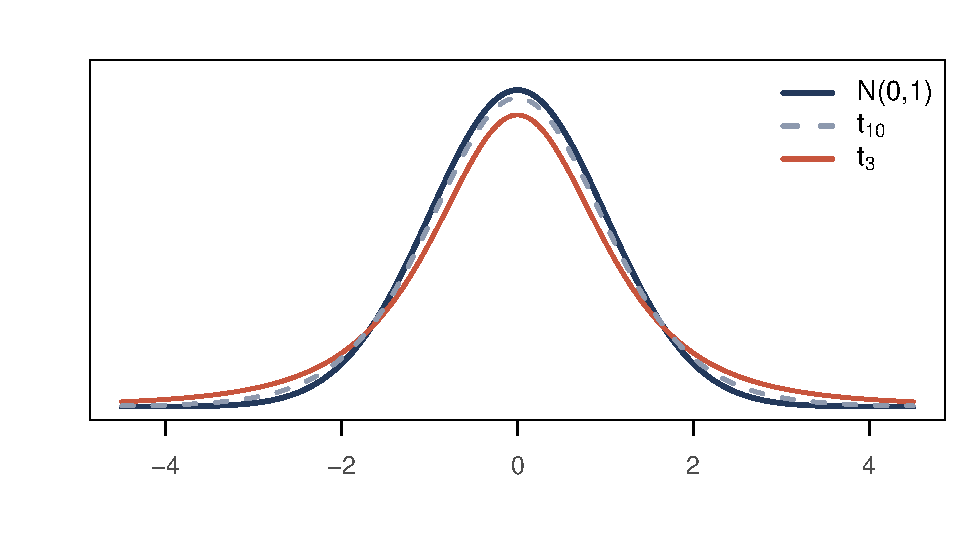
\includegraphics[width=1\linewidth,height=\textheight,keepaspectratio]{figs/t_vs_z.pdf}

}

\caption{\(t\) has fatter tails (extra uncertainty from estimating
\(\sigma\)); \(t_{10}\) is already close to \(N(0,1)\).}

\end{figure}%
\end{column}

\begin{column}{0.45\linewidth}
\begin{itemize}
\tightlist
\item
  Fatter tails \(\Rightarrow\) larger critical values: for 95\%,
  \(t_8=2.306\) vs \(z=1.96\).
\item
  As \(n-1\) grows, \(t_{n-1}\to N(0,1)\): \(t_{30}=2.042\),
  \(t_{120}=1.980\), \(t_\infty=1.960\).
\item
  With normal data, \(t\) is \textbf{never wrong}; for large \(n\) the
  two give practically the same interval, so we use \(z\).
\end{itemize}
\end{column}
\end{columns}
\end{frame}


\begin{frame}[shrink=5]{Critical values · \(z\) and \(t\) distributions}
\protect\phantomsection\label{critical-values-z-and-t}
\begin{columns}[T]
\begin{column}{0.33\textwidth}
\centering
\textbf{Standard normal \(z\)}\\[0.4em]
\footnotesize
\begin{tabular}{@{}ccc@{}}
\toprule
One-tailed \(\alpha\) & Two-tailed \(\alpha\) & Critical value \\
\midrule
0.10  & 0.20  & 1.282 \\
0.05  & 0.10  & 1.645 \\
0.025 & 0.05  & 1.960 \\
0.01  & 0.02  & 2.326 \\
0.005 & 0.01  & 2.576 \\
0.001 & 0.002 & 3.090 \\
\bottomrule
\end{tabular}
\end{column}

\begin{column}{0.63\textwidth}
\centering
\textbf{Student's \(t\)}\\[0.4em]
\scriptsize
\renewcommand{\arraystretch}{0.95}
\begin{tabular}{@{}r*{5}{r}@{}}
\toprule
One-tailed \(\alpha\) & 0.10 & 0.05 & 0.025 & 0.01 & 0.005 \\
Two-tailed \(\alpha\) & 0.20 & 0.10 & 0.05  & 0.02 & 0.01  \\
\midrule
df \(=1\) & 3.078 & 6.314 & 12.706 & 31.821 & 63.657 \\
2        & 1.886 & 2.920 & 4.303  & 6.965  & 9.925  \\
3        & 1.638 & 2.353 & 3.182  & 4.541  & 5.841  \\
4        & 1.533 & 2.132 & 2.776  & 3.747  & 4.604  \\
5        & 1.476 & 2.015 & 2.571  & 3.365  & 4.032  \\
8        & 1.397 & 1.860 & 2.306  & 2.896  & 3.355  \\
10       & 1.372 & 1.812 & 2.228  & 2.764  & 3.169  \\
15       & 1.341 & 1.753 & 2.131  & 2.602  & 2.947  \\
20       & 1.325 & 1.725 & 2.086  & 2.528  & 2.845  \\
25       & 1.316 & 1.708 & 2.060  & 2.485  & 2.787  \\
30       & 1.310 & 1.697 & 2.042  & 2.457  & 2.750  \\
40       & 1.303 & 1.684 & 2.021  & 2.423  & 2.704  \\
60       & 1.296 & 1.671 & 2.000  & 2.390  & 2.660  \\
120      & 1.289 & 1.658 & 1.980  & 2.358  & 2.617  \\
\midrule
\(\infty\) & 1.282 & 1.645 & 1.960 & 2.326 & 2.576 \\
\bottomrule
\end{tabular}
\end{column}
\end{columns}

\vspace{0.6em}
\centering\scriptsize Confidence intervals use the \textbf{two-tailed} row
(95\% CI \(\to\) two-tailed \(\alpha=0.05\)). The one-tailed row is for
one-sided tests (Section 4). As df \(\to\infty\), \(t\) converges to \(z\).
\end{frame}


\begin{frame}{Decision guide: which formula?}
\protect\phantomsection\label{decision-guide-which-formula}
\begin{enumerate}
\tightlist
\item
  Is \(\sigma\) \textbf{given} in the problem (not just \(s\)), and
  \(Y\) normal or \(n\) large? \(\to\) use \(\sigma\) and \(z\).
\item
  Otherwise we use \(s_{n-1}\). Is \(n\) large (say \(>30\))? \(\to\)
  use \(z\) (CLT).
\item
  Is \(n\) small? \(\to\) the data must be \textbf{normal}, and we use
  \(t_{n-1}\).
\end{enumerate}

\begin{block}{Then always}
\protect\phantomsection\label{then-always}
\begin{enumerate}
\tightlist
\item
  \textbf{Standard error:} \(\sigma/\sqrt n\) or \(\sqrt{s^2_{n-1}/n}\)
  (the root comes \emph{after} dividing by \(n\)).
\item
  \textbf{Critical value:} two-sided \(\Rightarrow\) quantile
  \(1-\alpha/2\) (95\% \(\to\) 0.975, \emph{not} 0.95).
\item
  \textbf{Margin} \(E=c\times\se\). Lower \(=\bar y-E\), upper
  \(=\bar y+E\), \textbf{width \(=2E\)}.
\end{enumerate}
\end{block}
\end{frame}


\begin{frame}{Worked example · a CI step by step}
\protect\phantomsection\label{worked-example-a-ci-step-by-step}
Hourly wage of young workers. Sample: \(n=100\), \(\bar y=20\) EUR,
\(s=5\) EUR. \(\sigma\) unknown, \(n\) large.

\begin{block}{Step by step}
\protect\phantomsection\label{step-by-step}
\begin{enumerate}
\tightlist
\item
  \textbf{Case:} \(\sigma\) unknown, \(n\) large \(\Rightarrow\) \(z\).
\item
  \textbf{SE:} \(s/\sqrt{n} = 5/\sqrt{100} = 5/10 =0.5\).
\item
  \textbf{Critical value, 95\%:} \(1.96\). \textbf{Margin:}
  \(1.96\times0.5=0.98\).
\item
  \textbf{CI:} \(20\pm0.98=[19.02,\ 20.98]\).
\end{enumerate}
\end{block}

\textbf{Reading it:} values of \(\mu\) between about 19 and 21 EUR/hour
are consistent with our data.

\textbf{What if we want 99\%?} Multiplier \(2.576\):
\(20\pm1.288=[18.71,\ 21.29]\). Wider: more confidence, less precision.
\end{frame}

\begin{frame}{Exercise 4: CI, unknown \(\sigma^2\), large sample}
\protect\phantomsection\label{exercise-4-ci-unknown-sigma2-large-sample}
The commuting time of workers in a city is studied. A random sample of
\(n=144\) workers gives \(\bar y=38.5\) minutes and \(s^2_{n-1}=324\).

\begin{enumerate}
\tightlist
\item
  Why can we use the normal approximation here, even without knowing the
  population distribution?
\item
  Compute the standard error.
\item
  Build a 95\% confidence interval for the mean commuting time.
\item
  What is its width?
\end{enumerate}

\emph{Hint:} follow the four steps of the worked example. Careful: the
variance is given, not the standard deviation.
\end{frame}

\begin{frame}{Solution Exercise 4}
\protect\phantomsection\label{solution-exercise-4}
\begin{enumerate}
\tightlist
\item
  \(n=144\) is large: by the CLT \(\bar y\) is approximately normal, and
  replacing \(\sigma\) by \(s_{n-1}\) is harmless in large samples.
\item
  \(\se(\bar y)=\sqrt{324/144}=\sqrt{2.25}=\mathbf{1.5}\) min.
\item
  \(z_{0.975}=1.96\):
  \[\bar y\pm1.96\times1.5=38.5\pm2.94=\mathbf{[35.56,\ 41.44]}\]
\item
  Width \(=2\times2.94=\mathbf{5.88}\) min.
\end{enumerate}

\textbf{Interpretation:} 95\% of intervals built this way contain the
true mean commute, which here is somewhere around 36 to 41 minutes.
\end{frame}

\begin{frame}{Exercise 5: CI with \emph{known} \(\sigma^2\)}
\protect\phantomsection\label{exercise-5-ci-with-known-sigma2}
A machine fills rice bags. Filled weights are normally distributed with
a \textbf{known} standard deviation \(\sigma=20\) g. A sample of
\(n=25\) bags has mean \(\bar y=502\) g.

\begin{enumerate}
\tightlist
\item
  Compute a 90\% confidence interval for the mean filled weight.
\item
  Compute a 99\% confidence interval. How does the width change, and
  why?
\end{enumerate}

\emph{Hint:} \(\sigma\) is given, so no \(s\) and no \(t\): the standard
error is \(\sigma/\sqrt n\).
\end{frame}

\begin{frame}{Solution Exercise 5}
\protect\phantomsection\label{solution-exercise-5}
Standard deviation of \(\bar y\) (no estimation needed):
\(\sigma/\sqrt n=20/5=4\) g. \\
Since \(Y\) is normal: Exact \(N(0,1)\)

\begin{enumerate}
\item
  90\%: \(z_{0.95}=1.645\):
  \(\ 502\pm1.645\times4=502\pm6.58=\mathbf{[495.42,\ 508.58]}\)
\item
  99\%: \(z_{0.995}=2.576\):
  \(\ 502\pm2.576\times4=502\pm10.30=\mathbf{[491.70,\ 512.30]}\)

  Width grows from 13.16 to 20.61: higher confidence \(\Rightarrow\)
  larger critical value \(\Rightarrow\) wider interval.
\end{enumerate}
\end{frame}

\begin{frame}{Exercise 6: CI in a small sample}
\protect\phantomsection\label{exercise-6-ci-in-a-small-sample}
The battery life (hours) of a new phone is assumed normally distributed.
A lab tests \(n=9\) phones: \(\bar y=11.2\) and \(s^2_{n-1}=2.25\).

\begin{enumerate}
\tightlist
\item
  Which distribution and which critical value should you use for a 95\%
  CI? Why not \(1.96\)?
\item
  Build the 95\% confidence interval.
\item
  Which of these critical values is right for \textbf{a 99\% CI with
  \(n=16\)}? \\ 
  (a) 2.576 \(\quad\) (b) 2.602 \(\quad\) (c) 2.947
  \(\quad\) (d) 2.131 \(\quad\) (e) 3.286
\end{enumerate}

\emph{Hint:} three ingredients for a critical value: which distribution,
which quantile (\(1-\alpha/2\)), how many degrees of freedom (\(n-1\)).
\end{frame}

\begin{frame}{Solution Exercise 6}
\protect\phantomsection\label{solution-exercise-6}
\begin{enumerate}
\item
  \(n=9\) is small and \(\sigma^2\) unknown \(\Rightarrow\)
  \(\dfrac{\bar y-\mu}{s/\sqrt n}\sim t_{8}\) (needs normal data).
  \(t_{8;\,0.975}=\mathbf{2.306}\). Using \(1.96\) would give an
  interval that is \textbf{too narrow}: it would cover \(\mu\) less than
  95\% of the time.
\item
  \(\se=\sqrt{2.25/9}=0.5\). Margin \(=2.306\times0.5=1.153\):
  \[11.2\pm1.153=\mathbf{[10.05,\ 12.35]}\] (With \(z\) it would wrongly
  be \([10.22,\ 12.18]\).)
\item
  Two-sided 99\% \(\Rightarrow\) \(1-\alpha/2=0.995\); \(df=n-1=15\)
  \(\Rightarrow\) \(t_{15;0.995}=\mathbf{2.947}\) \(\to\) \textbf{(c)}.

  \begin{enumerate}
  [(a)]
  \tightlist
  \item
    is the normal quantile; (b) is the one-sided \(t_{15;0.99}\); (d) is
    \(t_{15;0.975}\) (the 95\% value).
  \end{enumerate}
\end{enumerate}
\end{frame}


\begin{frame}{Margin of error and sample size}
\protect\phantomsection\label{margin-of-error-and-sample-size}
The margin of error of the interval is
\(E=z_{1-\alpha/2}\times\se(\bar y)=z_{1-\alpha/2}\sqrt{\sigma^2/n}\), so
for a fixed confidence level and population:

\[E\propto\frac{1}{\sqrt n}\]

\begin{itemize}
\tightlist
\item
  Precision grows with \(\sqrt n\), not with \(n\): to make \(E\)
  \textbf{\(k\) times smaller}, you need \(n'=n\times k^2\).
\item
  Intuition: a 3 times smaller margin needs 9 times more data.
\item
  Writing the ratio: \(\ E'/E=\sqrt{n/n'}=1/k\ \Rightarrow\ n'=k^2 n\).
\end{itemize}
\end{frame}

\begin{frame}{Exercise 7: Sample size}
\protect\phantomsection\label{exercise-7-sample-size}
\begin{enumerate}
\tightlist
\item
  A survey of \(n=150\) observations gives a CI with margin of error
  \(E=z_{1-\alpha/2}\,\se(\bar y)\). For the same population and
  confidence level, how large must the sample be for the margin of error
  to be \(E/3\)?
\item
  A poll with \(n=80\) has margin \(E\). What sample size gives a margin
  \(E/2\)?
\item
  The sample is doubled. By what factor does the width of the CI shrink?
\end{enumerate}

\emph{Hint:} \(E\propto1/\sqrt n\), so a \(k\)-fold smaller \(E\) needs
\(k^2\) times more data.
\end{frame}

\begin{frame}{Solution Exercise 7}
\protect\phantomsection\label{solution-exercise-7}
\begin{enumerate}
\item
  \(E'/E=\sqrt{n/n'}=1/3\Rightarrow n'=9n=150\times9=\mathbf{1350}\).
  Classic wrong answers: \(450\) (\(3n\)) or \(50\) (\(n/3\), which makes
  the interval \emph{wider}).
\item
  \(n'=2^2\times80=\mathbf{320}\).
\item
  \(\text{width}\propto1/\sqrt n\): doubling \(n\) shrinks the width by
  \(1/\sqrt2\approx0.71\), i.e.~only about \textbf{29\%} narrower.
\end{enumerate}
\end{frame}


\section{4. Hypothesis testing}\label{hypothesis-testing}

\begin{frame}{The logic of a test: a trial analogy}
\protect\phantomsection\label{the-logic-of-a-test-a-trial-analogy}
\begin{columns}[T]
\begin{column}{0.5\linewidth}
\textbf{A court case}

\begin{itemize}
\tightlist
\item
  Default: the defendant is \textbf{innocent} until proven guilty.
\item
  We convict only if the evidence is \textbf{very unlikely under
  innocence}.
\item
  Not guilty \(\neq\) proven innocent: maybe just not enough evidence.
\end{itemize}
\end{column}

\begin{column}{0.5\linewidth}
\textbf{A statistical test}

\begin{itemize}
\tightlist
\item
  Default: \(H_0\) is true (nothing special, e.g.~\(\mu=\mu_0\)).
\item
  We reject \(H_0\) only if the data would be \textbf{very unlikely if
  \(H_0\) were true}.
\item
  Not rejecting \(\neq\) proving \(H_0\): maybe just too little data.
\end{itemize}
\end{column}
\end{columns}

\begin{block}{The one question a test asks}
\protect\phantomsection\label{the-one-question-a-test-asks}
\emph{``If \(H_0\) were true, how surprising would my sample be?''} Very
surprising \(\Rightarrow\) we doubt \(H_0\).
\end{block}
\end{frame}

\begin{frame}{Setting up a test of the mean}
\protect\phantomsection\label{setting-up-a-test-of-the-mean}
\begin{itemize}
\tightlist
\item
  \textbf{Null} \(H_0:\ \mu=\mu_0\) (the claim being checked) vs an
  \textbf{alternative}: two-sided \(H_A:\mu\neq\mu_0\), or one-sided
  \(H_A:\mu>\mu_0\) / \(H_A:\mu<\mu_0\).
\item
  Fix the significance level \(\alpha\) (usually 5\%) \textbf{before}
  looking at the data: the false-alarm rate we tolerate.
\item
  \textbf{Test statistic} = \emph{signal-to-noise ratio}: how many
  standard errors is \(\bar y\) away from the claimed \(\mu_0\)?
  \[t=\frac{\bar y-\mu_0}{\se(\bar y)}=\frac{\text{signal: distance from }\mu_0}{\text{noise: typical sampling error}}\]
\item
  If \(H_0\) is true, \(t\sim N(0,1)\) (large \(n\)) or \(t_{n-1}\)
  (normal \(Y\), small \(n\)): the \textbf{null distribution}.
\item
  \(|t|\) close to 0: consistent with \(H_0\). \(|t|\) large: hard to
  explain by chance alone.
\end{itemize}
\end{frame}

\begin{frame}{Decision rule and p-value}
\protect\phantomsection\label{decision-rule-and-p-value}
\begin{itemize}
\item
  \textbf{p-value:} the probability, \textbf{assuming \(H_0\) is true},
  of a test statistic \emph{more extreme} than the one we observed.
\item
  \textbf{Significance level} \(\alpha\): a cutoff on the p-value,
  chosen \emph{before} the test. If \(p<\alpha\) we \textbf{reject}
  \(H_0\): what we observe is too unlikely under the Null.
\item
  \textbf{Equivalent rule (critical value):} reject if the observed
  statistic falls beyond the critical value.

  \begin{itemize}
  \tightlist
  \item
    two-sided \(H_A:\mu\neq\mu_0\): reject if \(|t|>c_{1-\alpha/2}\)
    (95\%: \(1.96\)).
  \item
    one-sided \(H_A\): ``more extreme'' means only the direction of
    \(H_A\) (right or left), and the critical value is \(c_{1-\alpha}\)
    (e.g.~\(1.645\)).
  \end{itemize}
\end{itemize}
\end{frame}

\begin{frame}{p-value: how surprising is my sample?}
\protect\phantomsection\label{p-value-how-surprising-is-my-sample}
\begin{columns}[T]
\begin{column}{0.52\linewidth}
\begin{figure}[H]

{\centering 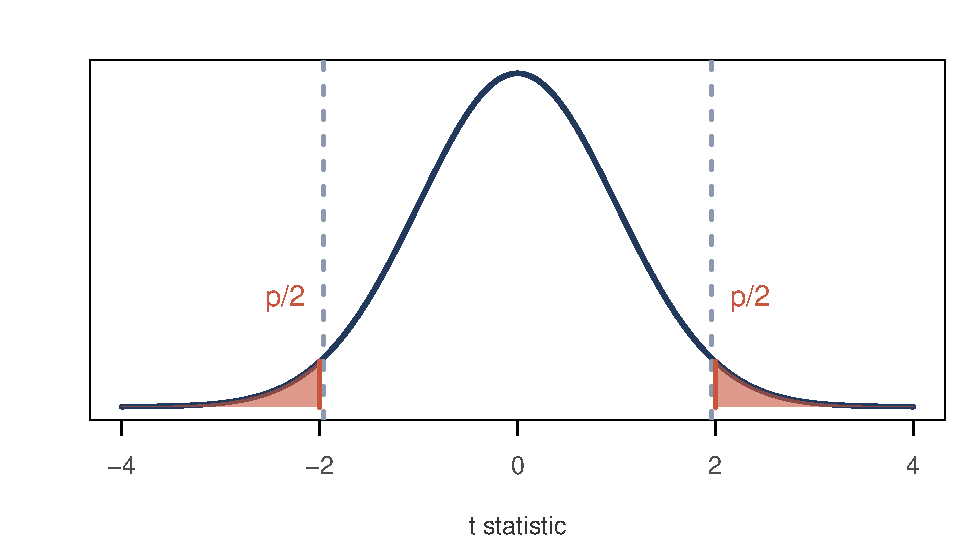
\includegraphics[width=1\linewidth,height=\textheight,keepaspectratio]{figs/pvalue.pdf}

}

\caption{Two-sided test, \(t=2.0\): p-value = red area (both tails).}

\end{figure}%
\end{column}

\begin{column}{0.48\linewidth}
\begin{itemize}
\tightlist
\item
  \textbf{p-value} = probability, \textbf{assuming \(H_0\) is true}, of
  getting a result \emph{at least as extreme} as ours.
\item
  Small p \(\Rightarrow\) our data would be rare under \(H_0\)
  \(\Rightarrow\) doubt \(H_0\).
\item
  \textbf{Reject \(\iff\) \(p<\alpha\) \(\iff\) \(|t|>\) critical
  value.} Two routes, same decision.
\end{itemize}
\end{column}
\end{columns}
\end{frame}

\begin{frame}{Worked example · a test step by step}
\protect\phantomsection\label{worked-example-a-test-step-by-step}
Does the average student sleep \textbf{8 hours}? Sample: \(n=100\),
\(\bar y=7.7\) h, \(s=3\) h.

\begin{block}{Step by step}
\protect\phantomsection\label{step-by-step-1}
\begin{enumerate}
\tightlist
\item
  \textbf{Hypotheses:} \(H_0:\mu=8\) vs \(H_A:\mu\neq8\). Choose
  \(\alpha=5\%\).
\item
  \textbf{SE:} \(3/\sqrt{100}=0.3\).
\item
  \textbf{Test statistic:} \(t=\dfrac{7.7-8}{0.3}=-1.0\): the sample is
  only \textbf{one SE} below 8.
\item
  \textbf{Decide:} \(|t|=1.0<1.96\). p-value
  \(=2\times\Pr(Z>1)=0.317>0.05\) \(\Rightarrow\) \textbf{do not
  reject}.
\item
  \textbf{In words:} a gap of 0.3 h is well within normal sampling
  noise. We \textbf{fail to reject} \(H_0\): no evidence against 8 hours
  (like ``not guilty'': that does not prove it is exactly 8).
\end{enumerate}
\end{block}
\end{frame}

\begin{frame}{Errors, power, and the role of \(\alpha\)}
\protect\phantomsection\label{errors-power-and-the-role-of-alpha}
\begin{columns}[T]
\begin{column}{0.5\linewidth}
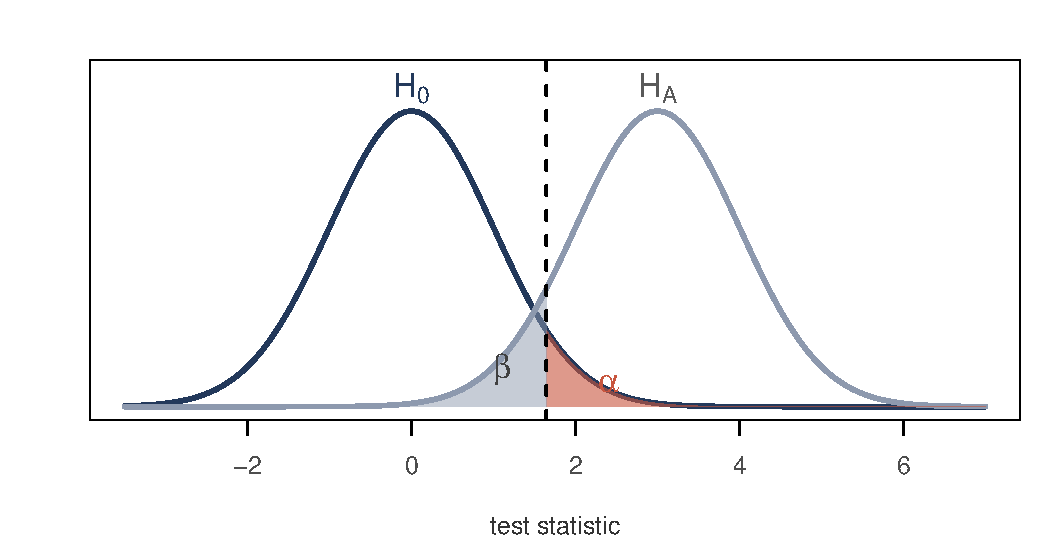
\includegraphics[width=1\linewidth,height=\textheight,keepaspectratio]{figs/errors.pdf}

\textbf{Power} \(=1-\beta\): probability of \emph{not} making a Type II
error.
\end{column}

\begin{column}{0.5\linewidth}
{\def\LTcaptype{none} % do not increment counter
\begin{longtable}[]{@{}lll@{}}
\toprule\noalign{}
& \(H_0\) true & \(H_0\) false \\
\midrule\noalign{}
\endhead
Reject & Type I (\(\alpha\)) & power \(1-\beta\) \\
Keep & correct & Type II (\(\beta\)) \\
\bottomrule\noalign{}
\end{longtable}
}

\begin{itemize}
\tightlist
\item
  \textbf{Type I} = false alarm; \textbf{Type II} = missed detection.
\item
  We \textbf{choose} \(\alpha\); \(\beta\) depends on the true \(\mu\),
  \(n\), \(\sigma\).
\item
  Lower \(\alpha\) \(\Rightarrow\) cutoff moves right \(\Rightarrow\)
  \(\beta\) up.
\item
  The two errors are inversely related: we fix \(\alpha\) and try to
  maximise the power.
\end{itemize}
\end{column}
\end{columns}
\end{frame}

\begin{frame}{Exercise 8: Two-sided test, large sample}
\protect\phantomsection\label{exercise-8-two-sided-test-large-sample}
A delivery company claims that its \textbf{average delivery time is 30
minutes}. You check \(n=225\) random orders and find \(\bar y=31.2\) min
and \(s^2_{n-1}=81\).

\emph{Question:} is the data compatible with the company's claim?

\begin{enumerate}
\tightlist
\item
  Write \(H_0\) and \(H_A\). (The claim could be wrong in either
  direction, so use a two-sided test.)
\item
  Compute the standard error \(\se(\bar y)=s/\sqrt n\).
\item
  Compute the test statistic \(t=\dfrac{\bar y-30}{\se(\bar y)}\).
\item
  Decide: reject \(H_0\) at \(\alpha=5\%\)? And at \(\alpha=1\%\)?
\item
  Compute the p-value and check it agrees with step 4.
\end{enumerate}

\emph{Hints:} \(s^2=81\Rightarrow s=9\). Large \(n\), so use \(z\)
critical values. p-value \(=2\,(1-\Phi(|t|))\), where
\(\Phi(z)=\Pr(Z\le z)\); you may use \(\Phi(2.00)=0.9772\).
\end{frame}

\begin{frame}{Solution · Exercise 8}
\protect\phantomsection\label{solution-exercise-8}
\begin{enumerate}
\tightlist
\item
  \(H_0:\mu=30\ \) vs \(\ H_A:\mu\neq30\).
\item
  \(\se=9/\sqrt{225}=9/15=\mathbf{0.6}\) min.
\item
  \(t=\dfrac{31.2-30}{0.6}=\mathbf{2.00}\): the sample mean is 2
  standard errors above the claim.
\item
  \(\alpha=5\%\): \(|t|=2.00>1.96\) \(\Rightarrow\) \textbf{reject}
  \(H_0\). \(\quad\) \(\alpha=1\%\): \(2.00<2.576\) \(\Rightarrow\)
  \textbf{do not reject}.
\item
  p-value \(=2\,(1-0.9772)=\mathbf{0.0456}\): smaller than 0.05, larger
  than 0.01. Same decisions as step 4. \(\checkmark\)
\end{enumerate}

\textbf{In words:} at 5\% the data are too unlikely if the true mean were
30 minutes, so we doubt the claim. But the evidence is borderline: with a
stricter \(\alpha=1\%\) we would not reject.
\end{frame}

\begin{frame}{Exercise 9 · The small-sample trap}
\protect\phantomsection\label{exercise-9-the-small-sample-trap}
A lab sets the target mean strength of a cable at \(\mu_0=100\). The
strength is normally distributed. A sample of \(n=9\) cables gives
\(\bar y=106.6\) and \(s^2_{n-1}=81\).

\begin{enumerate}
\tightlist
\item
  Compute the \(t\)-statistic for \(H_0:\mu=100\) vs \(H_A:\mu\neq100\).
\item
  Decide at 5\% using (i) the normal critical value and (ii) the correct
  one. Do they agree?
\item
  Which is correct and why?
\end{enumerate}

\emph{Hint:} \(n=9\) \(\Rightarrow\) degrees of freedom \(=8\)
(\(t_{8;0.975}=2.306\)).
\end{frame}

\begin{frame}{Solution · Exercise 9}
\protect\phantomsection\label{solution-exercise-9}
\begin{enumerate}
\tightlist
\item
  \(\se=\sqrt{81/9}=3\), \(\quad t=\dfrac{106.6-100}{3}=\mathbf{2.20}\).
\item
  \begin{enumerate}
  [(i)]
  \tightlist
  \item
    Normal: \(2.20>1.96\) \(\Rightarrow\) reject.
  \item
    \(t_{8;0.975}=2.306\): \(2.20<2.306\) \(\Rightarrow\) \textbf{fail
    to reject}.
  \end{enumerate}
\item
  Only (ii) is valid: \(n=9\) is small and \(\sigma\) is estimated, so
  the statistic follows \(t_8\). The normal quantile is too small for a
  small sample and would reject too often.
\end{enumerate}
\end{frame}

% \begin{frame}{Exercise 10 · True or false?}
% \protect\phantomsection\label{exercise-10-true-or-false}
% \begin{enumerate}
% \tightlist
% \item
%   ``Rejecting \(H_0\) when it is true is a Type II error.''
% \item
%   ``The sample mean is an unbiased estimator of \(\mu\) only if \(Y\) is
%   normally distributed.''
% \item
%   ``If we fail to reject \(H_0\), then \(H_0\) is true.''
% \item
%   ``Doubling the sample size halves the margin of error.''
% \item
%   ``With \(n=200\) and a clearly skewed \(Y\) we cannot use the normal
%   critical value.''
% \item
%   ``Lowering \(\alpha\) makes a Type II error more likely.''
% \end{enumerate}
% \end{frame}

% \begin{frame}{Solution · Exercise 10}
% \protect\phantomsection\label{solution-exercise-10}
% \begin{enumerate}
% \tightlist
% \item
%   \textbf{False.} That is a Type I error (convicting an innocent). Type
%   II = failing to reject a wrong \(H_0\).
% \item
%   \textbf{False.} \(E(\bar y)=\mu\) whenever the \(y_i\) are i.i.d.: no
%   normality needed.
% \item
%   \textbf{False.} Like ``not guilty'' is not ``innocent'': we only
%   lacked enough evidence to reject.
% \item
%   \textbf{False.} \(E\propto1/\sqrt n\): the margin shrinks by
%   \(1/\sqrt2\); to halve it, \(n\) must be \textbf{quadrupled}.
% \item
%   \textbf{False.} The CLT makes \(\bar y\) approximately normal for
%   large \(n\), whatever the distribution of \(Y\).
% \item
%   \textbf{True.} Type I and II errors are inversely related: a smaller
%   \(\alpha\) moves the critical value outwards and raises \(\beta\).
% \end{enumerate}
% \end{frame}

\section{5. Wrap-up}\label{wrap-up}

\begin{frame}{Summary}
\protect\phantomsection\label{the-whole-session-in-one-picture}
\begin{block}{One recipe for everything}
\protect\phantomsection\label{one-recipe-for-everything}
\[\frac{\text{estimate}-\text{benchmark}}{\text{standard error}}\ \text{ is compared with a } z \text{ or } t \text{ table}\]
\end{block}

\begin{itemize}
\tightlist
\item
  \textbf{Confidence interval:} start from the estimate, go \(\pm\)
  (critical value) \(\times\) SE. \(\Rightarrow\) \emph{plausible values
  of \(\mu\)}.
\item
  \textbf{Hypothesis test:} measure how many SE the estimate is from the
  claim \(\mu_0\). \(\Rightarrow\) \emph{is the claim plausible?}
\item
  \textbf{Same ingredients:} \(\bar y\), \(\se=s/\sqrt n\), and the
  critical value (\(z\) for large \(n\) or known \(\sigma\); \(t_{n-1}\)
  for small \(n\) with unknown \(\sigma\)).
\item
  \textbf{CLT} is what makes all this work for non-normal data when
  \(n\) is large.
\end{itemize}
\end{frame}

\begin{frame}{Cheat sheet}
\protect\phantomsection\label{cheat-sheet}
{\def\LTcaptype{none} % do not increment counter
\begin{longtable}[]{@{}
  >{\raggedright\arraybackslash}p{(\linewidth - 4\tabcolsep) * \real{0.2447}}
  >{\raggedright\arraybackslash}p{(\linewidth - 4\tabcolsep) * \real{0.3085}}
  >{\raggedright\arraybackslash}p{(\linewidth - 4\tabcolsep) * \real{0.4468}}@{}}
\toprule\noalign{}
\begin{minipage}[b]{\linewidth}\raggedright
\end{minipage} & \begin{minipage}[b]{\linewidth}\raggedright
\textbf{Confidence interval}
\end{minipage} & \begin{minipage}[b]{\linewidth}\raggedright
\textbf{Test of \(H_0:\mu=\mu_0\)}
\end{minipage} \\
\midrule\noalign{}
\endhead
\(\sigma^2\) known & \(\bar y\pm z\,\sigma/\sqrt n\) &
\(z=(\bar y-\mu_0)\,/\,(\sigma/\sqrt n)\) \\
\(\sigma^2\) unknown, large \(n\) & \(\bar y\pm z\,s/\sqrt n\) &
\(t=(\bar y-\mu_0)\,/\,(s/\sqrt n)\approx N(0,1)\) \\
\(\sigma^2\) unknown, small \(n\), normal \(Y\) &
\(\bar y\pm t_{n-1}\,s/\sqrt n\) &
\(t=(\bar y-\mu_0)\,/\,(s/\sqrt n)\sim t_{n-1}\) \\
\bottomrule\noalign{}
\end{longtable}
}

\begin{itemize}
\tightlist
\item
  \(z_{0.95}=1.645,\ z_{0.975}=1.96,\ z_{0.995}=2.576\) \(\quad\) ·
  \(\quad\) width \(=2\times\) margin
\item
  Reject \(\iff\) \(p<\alpha\) \(\iff\) \(|t|>c_{1-\alpha/2}\)
  (two-sided) \(\quad\) · \(\quad\) \(E\propto1/\sqrt n\)
\end{itemize}
\end{frame}

\end{document}
